\documentclass[]{article}

\usepackage{graphicx}
\newcommand{\avval}[1]{\langle #1 \rangle}

%opening
\title{Physics 319 Final Project: Magnetic Field Mapper}
\author{Phillip Bement}

\begin{document}

\maketitle

\begin{abstract}
TODO
\end{abstract}


\section*{Introduction}

The purpose of this project is to be able to measure and map out what a magnetic field looks like in space. For example, if you are designing a motor with permanent magnets in it, it would be useful to see what the magnetic field looks like around those magnets. In a broader context, people have mapped the magnetic field of the Earth, in order to allow ships to determine true north from the direction of their compasses.

% TODO: fix this

\section*{Theory}

To measure the magnetic field, we use devices known as Hall effect sensors. The Hall effect happens when a current is passed through a conductor in the presence of a magnetic field.

\begin{figure}
\begin{center}
% TODO: cite
\caption{This diagram shows an example of the Hall effect in action. \label{fig:hall}}
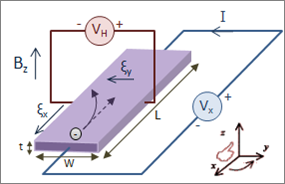
\includegraphics[width=.9\linewidth]{Hall_Effect_Measurement_Setup_for_Electrons}
\end{center}
\end{figure}

The effect happens because the carriers of current, (i.e. electrons in many materials) must have an average velocity in order to carry current, and this in turn means that there is an average Lorentz force acting on them. See figure~\ref{fig:hall} for a diagram of how this works.

Here is a more detailed explanation: Suppose that each charge carrier has a charge of $e$, and these carriers have a density of $n$ in the conductor. (So there are $nV$ carriers on average in a volume $V$ of conductor.) Suppose that the conductor is shaped like a rectangular prism as in figure~\ref{fig:hall}, and that the cross sectional area of this prism through which the current is flowing is $A$. (So $A$ would be the area of the rectangular prism if sliced through the $z$-$y$ plane in the figure.) If $\vec I$ is the current flowing through the conductor, then $I = neA\avval{\vec  v}$, where $\avval{\vec  v}$ is the average velocity of a charge carrier. Therefore:

$$
\avval {\vec  v} = \frac{1}{ne}\frac{\vec I}{A} = \frac{1}{ne} \vec J
$$

(Where $\vec J$ is current density.)

Now, suppose that we set up a device as in figure~\ref{fig:hall} so that there is a current flowing in the $x$ direction, and we measure voltage in the $y$ direction. Also, suppose that our voltage measuring device has a large resistance, so that $\vec I = I \hat x$. Then this implies that $\avval{\vec v}$ is also in the $\hat x$ direction. i.e. $\avval{\vec v} = \avval{v_x}\hat x$. Thus, the average resistive force on charge carriers is also in the $\hat x$ direction.

Suppose that the $\vec B$ field is in the $z$ direction, so that $\vec B = B\hat z$. Then there will be an average Lorentz force on the charge carriers of:

$$
\avval {\vec F_B} = e \avval v \times \vec B = e \avval{v_x} B \hat x \times \hat z = - e \avval{v_x} B \hat y
$$

When the current is first turned on, this force will rapidly cause the charge carriers to move to one side, piling up on one side of the conductor, and depleting on the other. This movement will produce an electric field, however, which will soon cancel the effect, resulting in zero average force on the charge carriers in the conductor. So we will have $\avval {F_{E,y}} = eE_y = -\avval{F_{B,y}} = e \avval{v_x} B$. And if we put in our result for $\avval {v_x}$, we get: $E_y =  \frac{1}{ne}\frac{I}{A} B$. If $w$ is the width of the conductor in the $y$ direction, and $t$ is its thickness in the $z$ direction, as shown in figure \ref{fig:hall}, then we have:

$$
A = tw
$$

$$
V_H = E_yw
$$

Where $V_H$ is the Hall voltage. Therefore:

$$
V_H = \frac{1}{ne}\frac{I}{t} B
$$

To take some typical examples of these values, suppose that the charge carriers are electrons, in a thin sample of Lithium metal. Suppose that $t = 1 \mu m$, and $I = 1mA$, and $B=0.01T$. Lithium has one carrier electron per atom, a density of $534kg/m^3$, and an atomic mass of $1.15 \cdot 10^{-26}kg$. Thus, its carrier density is $n = 534 / (1.15 \cdot 10^{-26}) m^{-3} = 4.64\cdot 10^{28} m^{-3}$. Therefore:

$$
V_H = \frac{1}{4.64\cdot 10^{28} m^{-3} \cdot 1.6 \cdot 10^{-19} C} \cdot \frac{1\cdot 10^{-3} A}{1\cdot {10^{-6}} m} \cdot 1 \cdot 10^{-2} T
$$

$$
= 1.35\cdot 10^{-9} V
$$

So for most cases, this is an extremely tiny effect. You can make it larger by using a conductor with a much lower carrier density, howevwer.

The Hall effect sensors that I use, the A1302's, have an apparatus much like that shown in figure~\ref{fig:hall} inside of them, along with an amplifier, to magnify the measly Hall voltage that is produced. They are designed to have a linear response to magnetic field, which makes calculating the field from the measured voltage much easier.

\section*{Apparatus}

The basic design of the device was to have three Hall effect sensors on the end of an arm. I call this the "sensor arm". The sensor arm was controlled by servo motors to determine its position and orientation in space, and the Hall effect sensors measured the value of the magnetic field at its tip. (The Hall sensors can each measure the field in only one direction, so three are required.) By analogy with spherical coordinates, I call the unit vectors that I measure the field along $r$, $\phi$, and $\theta$. Converting these vectors to Cartesian coordinates has the exact same formula as in converting spherical coordinates to Cartesian coordinates, so these names are useful. The two servo motors control the azimuth of the arm (which way it is pointing horizontally, corresponding to $\phi$) and the altitude (how vertical the arm is, corresponding to $\theta$).

\begin{figure}
\begin{center}
\caption{This diagram shows the sensor arm and the sensors pointing in 3 perpendicular directions. \label{fig:axes}}
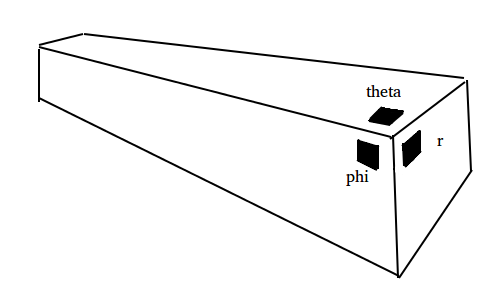
\includegraphics[width=.9\linewidth]{sensor_axes}
\end{center}
\end{figure}

\begin{figure}
\begin{center}
\caption{This diagram shows a view of the device from above. (not to scale) \label{fig:topv}}
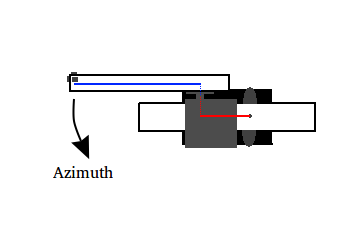
\includegraphics[width=.9\linewidth]{top_view}
\end{center}
\end{figure}

\begin{figure}
\begin{center}
\caption{This diagram shows a view of the device from the side. (not to scale) \label{fig:sidev}}
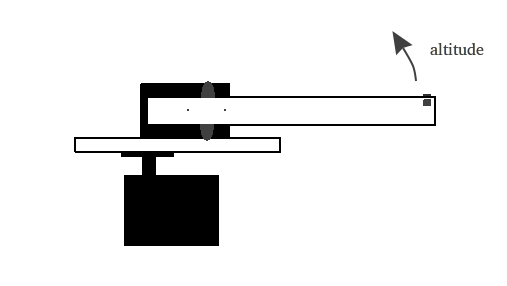
\includegraphics[width=.9\linewidth]{side_view}
\end{center}
\end{figure}

However, the end of the arm does not trace out a sphere in space. The axes of rotation for the two motors do not intersect, so rotating the azimuth motor actually changes the position of the altitude motor. This can be seen from the top view diagram, figure~\ref{fig:topv}. This means that the shape traced out in space is a torus, though a self intersecting one.

A torus has two radii. Call them $R$ and $r$. If we view a torus a being a circle rotated about some axis, then $r$ would be the radius of the original circle, while $R$ would be the distance from the center of that circle to the axis of rotation. In figure~\ref{fig:topv}, $r$ is the  blue line, while $R$ is the red line.

\begin{figure}
\begin{center}
\caption{Computing the cartesian coordinates. \label{fig:trig}}
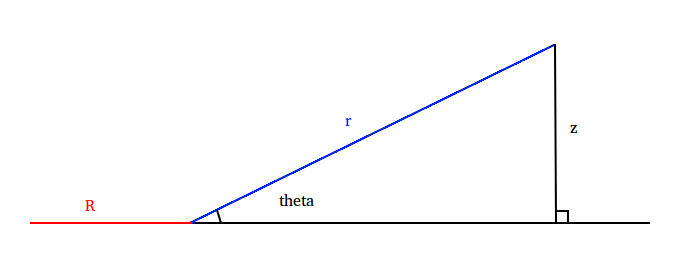
\includegraphics[width=.9\linewidth]{triangle}
\end{center}
\end{figure}

As we can see from figure~\ref{fig:trig}, this means that the value of $z$ will be $r \sin \theta$, while the value of $\sqrt{x^2+y^2}$ will be $R + r\cos\theta$. Factoring in $\phi$ to tell us what the $x$ and $y$ components should be gives us:

$$
x = (R + r\cos\theta)\cos \phi
$$

$$
y = (R + r\cos\theta)\sin \phi
$$

$$
z = r\sin\theta
$$

This now tells us exactly what the position of the end of the sensor arm and value of the magnetic field there will be in Cartesian coordinates.

Using the magnetic field mapper is not too difficult: the MSP430 microcontroller is powered by a USB cable to a computer. The rest of the project is powered by the lab 5V power supply, since both the servos and the Hall sensors can be powered  by 5V. After flashing the compiled {\tt scan.c} program onto the microcontroller, the user starts a python program called {\tt read\_data.py}. This program reads data sent over the USB cable from the microcontroller, does a small amount of processing, and saves it to a csv file. The microcontroller, meanwhile, after waiting a small amount of time for the user to start the python program, does the work of moving the arm to various locations in space, measuring the field, and sending the collected data to the computer.

\end{document}
